\chapter{Data processing for OCR}
\label{sec:Data processing for OCR}
An overview of the system that has been used for when using random forest for OCR is illustrated in figure \ref{system OCR}. The system has two different classifier. The first one is trained for separating background from characters and is used with less features than the second classifier. This classifier only has two different classes, false for background and true for characters. The second classifier is used to classify individual characters, it is used with an arbitrary number of classes depending on how many different characters that has been used during training.
%Flow chart
\begin{figure}[H]
\centering
\tikzstyle{largeblock} = [rectangle, draw, fill=blue!20, 
    text width=10em, text centered, rounded corners, minimum height=5em]
\tikzstyle{block} = [rectangle, draw, fill=blue!20, 
    text width=6em, text centered, rounded corners, minimum height=4em]
\tikzstyle{line} = [draw, -latex']
\tikzstyle{cloud} = [draw, ellipse,fill=red!20, node distance=3cm,
    minimum height=2em]
 
\begin{tikzpicture}[node distance = 2.5cm, auto]
    % Place nodes
    \node [cloud] (trainingImage) {training data};
    \node [largeblock, below of=trainingImage] (trainingData1) {produce training data and extract features};
    \node [largeblock, below of=trainingData1, node distance=7.5cm] (machine1) {training using Random forest};


     \node [cloud, right of=trainingImage, node distance=4cm] (trainingBack) {training data};
     \node [largeblock, below of=trainingBack] (trainingData2) {produce training data and extract features};
      \node [largeblock, below of=trainingData2] (machine2) {training using Random forest};
     
    \node [cloud, right of=trainingBack, node distance=4cm] (test) {test data};
    \node [block, below of=test] (features1) {extract features};
    \node [block, below of=features1] (classifier1) {Classifier 1};
    \node [block, below of=classifier1] (feature2) {extract features};
    \node [block, below of=feature2] (classifier2) {classifier 2};
    \node [block, below of=classifier2] (prediction) {prediction};
    
    
    % Draw edges
    \path [line] (trainingImage) -- (trainingData1);
    \path [line] (trainingData1) -- (machine1);
    \path [line] (trainingBack) -- (trainingData2);
     \path [line] (trainingData2) -- (machine2);
    \path [line] (machine2) -- (classifier1);
    \path [line] (machine1) -- (classifier2);
    \path [line] (test) -- (features1);
    \path [line] (features1) -- (classifier1);
    \path [line] (classifier1) -- (feature2);
    \path [line] (feature2) -- (classifier2);
    \path [line] (classifier2) -- (prediction);

\end{tikzpicture}
\caption{Overview of the system for OCR}
\label{system OCR}
\end{figure}

\section{Preprocessing of dataset}
\label{sec:Preprocessing of dataset}
The dataset used for training classifiers for character recognition are produced from sample images, one for each character. In this project a special font, OCR-A, has been used. This font has been particularly designed for OCR in a way that makes the character as dissimilar to each other as possible.

\begin{figure}[H]
\centering
	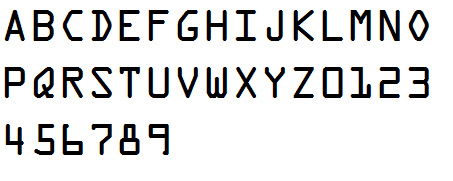
\includegraphics[scale=0.5]{OCRAfont}
	\caption{Image illustrating OCR A-font}
	\label{Afont}
\end{figure}

From these images a large dataset is produced. This is done by randomly changing the images in different ways depending on what kind of features that will be used later. Every training sample are first resized to the tile size, 54 times 64 pixels. The reason for choosing this size is because all characters are a bit larger in height than in width. An other reason is that the characters normally are written in lines and if the tile is too wide it will enclose more then one character. 

The character is then translated  and rotated randomly  in a way that it still remain entirely inside the tile. Depending what kind of features that are used for the classifier there are some more variations that can be applied to the training samples. Some random noise can be added to the samples. There can also be some variation of the thickness on the characters. This can be done by randomly eroding or dilating the sample images. In figure \ref{OCRSample3} two examples of training samples are illustrated for the character 3. The Samples have been translated, rotated and some thinning or thickening have been applied.

\begin{figure}[H]
\centering
	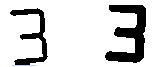
\includegraphics[scale=1]{OCRSample33}
	\caption{Image illustrating two different training samples of the character 3}
	\label{OCRSample3}
\end{figure}

Every character will also be assigned a class label. For example all training samples representing an A will have the class label A. If the characters are written on a line the classifier often make false detections between the characters and also above and under the character. Hence one false class have been added to the training. The training samples for the false class are produced by picking one or two random characters and putting them somewhere at the edge of the tile. In figure \ref{OCRSampleFalse} there is an example of a false sample.

\begin{figure}[H]
\centering
	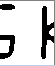
\includegraphics[scale=1]{OCRSampleFalse}
	\caption{Image illustrating an example of a false class}
	\label{OCRSampleFalse}
\end{figure}

\subsection{Character and background separation}
\label{sec:Character and background separation}
The classifier which separates background and characters  is using the same kind of images for training which was described in section \ref{sec:Preprocessing of dataset} above. In addition random background images are produced and divided into tiles, see figur...

%bild

The tiles from the random background images are then labeled as false. The tiles containing characters are labeled as true and tiles containing parts of images illustrated in figure \ref{OCRSampleFalse} are labeled as false.
  

\section{Postprocessing}
\label{sec:Postprocessing}

